\chapter{Diagrama de Classes} \label{cha:diagramaclasses}

O diagrama de classes apresentado neste capítulo oferece uma representação visual das entidades e relacionamentos fundamentais que compõem a estrutura do aplicativo. Cada classe no diagrama representa um tipo de objeto no sistema, como produtos, localizações e usuários. Os atributos de cada classe são detalhados, fornecendo informações sobre as características e comportamentos dos objetos representados. 

Além disso, as associações entre as classes indicam as interações entre os objetos, como a relação entre produtos e localizações, usuários e produtos favoritos. O diagrama de classes é uma ferramenta valiosa para entender a estrutura e o funcionamento interno do aplicativo, auxiliando no desenvolvimento, manutenção e evolução do sistema ao longo do tempo.



%DUVIDA: explicação pro diagram?

\imagem{DIAGRAMA DE CLASSES}{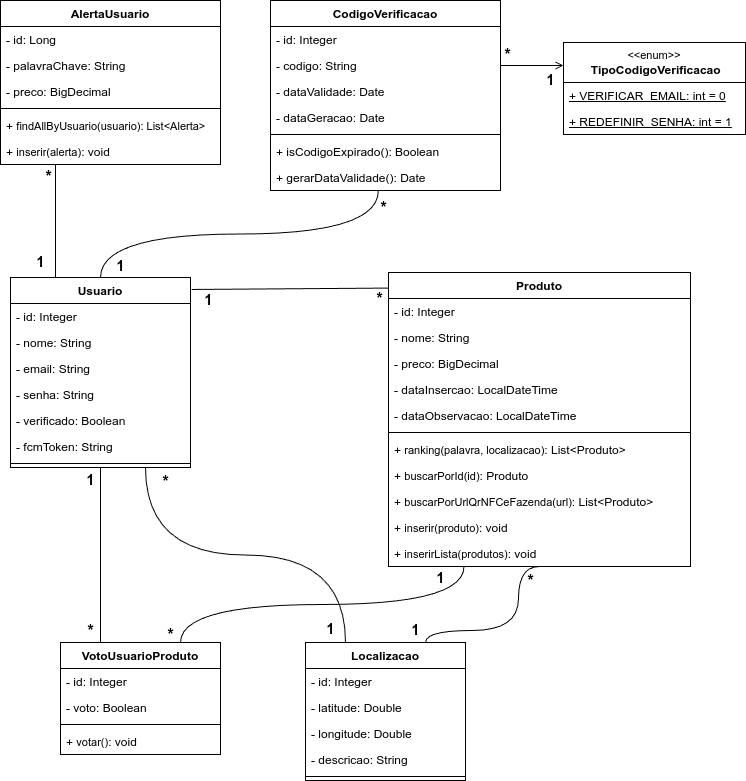
\includegraphics[width = 170mm]{fig/class.png}}{O Autor (2024)}{class}{nota(s)}{legenda(s)}